% Figure environments and legends of the retrieval figures, generated by
% python -m pmc_pair_retrieval.figures from the source data in source_data/.
% Every figure is 180 mm wide (85.5 to 207.2 mm high) and must be included at 100%, so
% that all of its text stays at 7 pt: the text block must be at least 180 mm wide (on A4, side
% margins of 15 mm or less). Any reduction must be applied equally to every figure, and the
% resulting text size stated. Each figure fits on one page with its legend directly below it in the
% reference layout of figure_pages.tex: A4 with 15 mm margins (text block 180 x 267 mm), legends
% in 8 pt.
% Requires \usepackage{graphicx} and \usepackage{url}; the citations of the example legends
% refer to the entries of image_references.tex.

\begin{figure}[p]
\centering
\makebox[\linewidth][c]{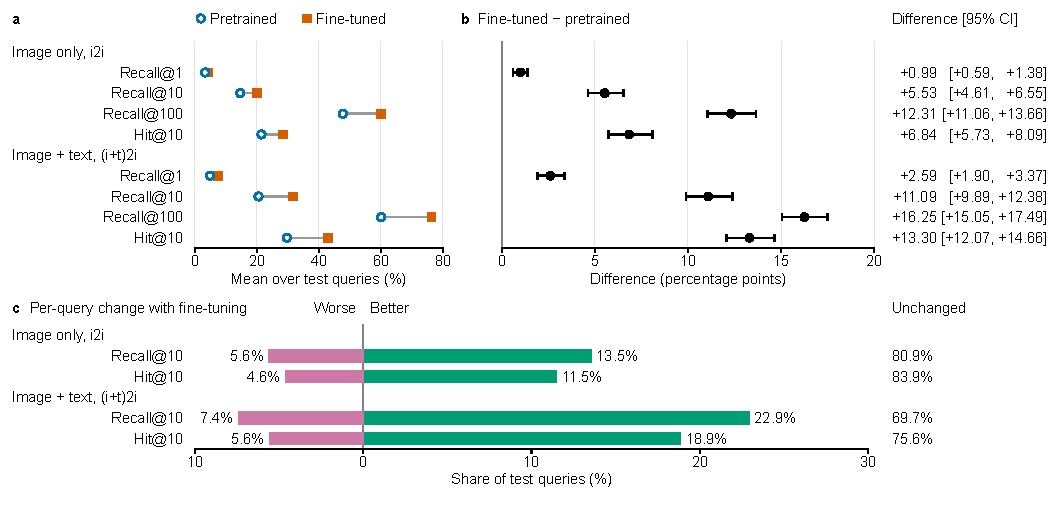
\includegraphics{retrieval_performance.pdf}}
\caption[Retrieval performance of pretrained and fine-tuned BiomedCLIP on the 8,096 test queries.]{Retrieval performance of pretrained and fine-tuned BiomedCLIP on the 8,096 test queries. Every test image is a query, the other 8,095 test images form the gallery, and the images recorded as pair partners of the query (recorded positives) are the relevant images; images linked to the query only through a chain of pairs are left out of its ranking. Both models encode every image from three $224 \times 224$ pixel views. i2i, image-only queries (configuration image\_to\_image), scored by the cosine similarity of the query and gallery image embeddings; (i+t)2i, image-plus-text queries (configuration image\_text\_to\_image), scored by that cosine similarity plus the dot product of the gallery image embedding with the mean (not renormalized) of the unit text embeddings of the query image's distinct descriptions. Fine-tuned, the released weights of each configuration, from the epoch with the highest validation Recall@10 (i2i, epoch 11 of 12; (i+t)2i, epoch 21 of 30, with the mean-description query text). \textbf{a}, Mean Recall@k (share of a query's recorded positives among its k highest-ranked images) for k = 1, 10 and 100, and Hit@10 (share of queries with a recorded positive in the top 10), in percent; symbols as in the key. \textbf{b}, Mean paired difference, fine-tuned minus pretrained, in percentage points, with 95\% confidence intervals (CI) from a query-weighted bootstrap over the 1,335 article groups of the test split (articles connected by recorded pairs; 5,000 resamples; percentile intervals); Recall@10: +5.53 [+4.61, +6.55] for i2i and +11.09 [+9.89, +12.38] for (i+t)2i. \textbf{c}, Share of queries whose Recall@10 or Hit@10 is higher (better, bars to the right) or lower (worse, bars to the left) with the fine-tuned than with the pretrained model; the column at the right gives the share with equal values under both models (unchanged). Shares are rounded to one decimal and may not sum to 100\%. Most unchanged queries have no recorded positive in the top 10 of either model (5,429 of 6,546 for i2i and 4,166 of 5,641 for (i+t)2i, Recall@10).}
\label{fig:retrieval-performance}
\end{figure}

\begin{figure}[p]
\centering
\makebox[\linewidth][c]{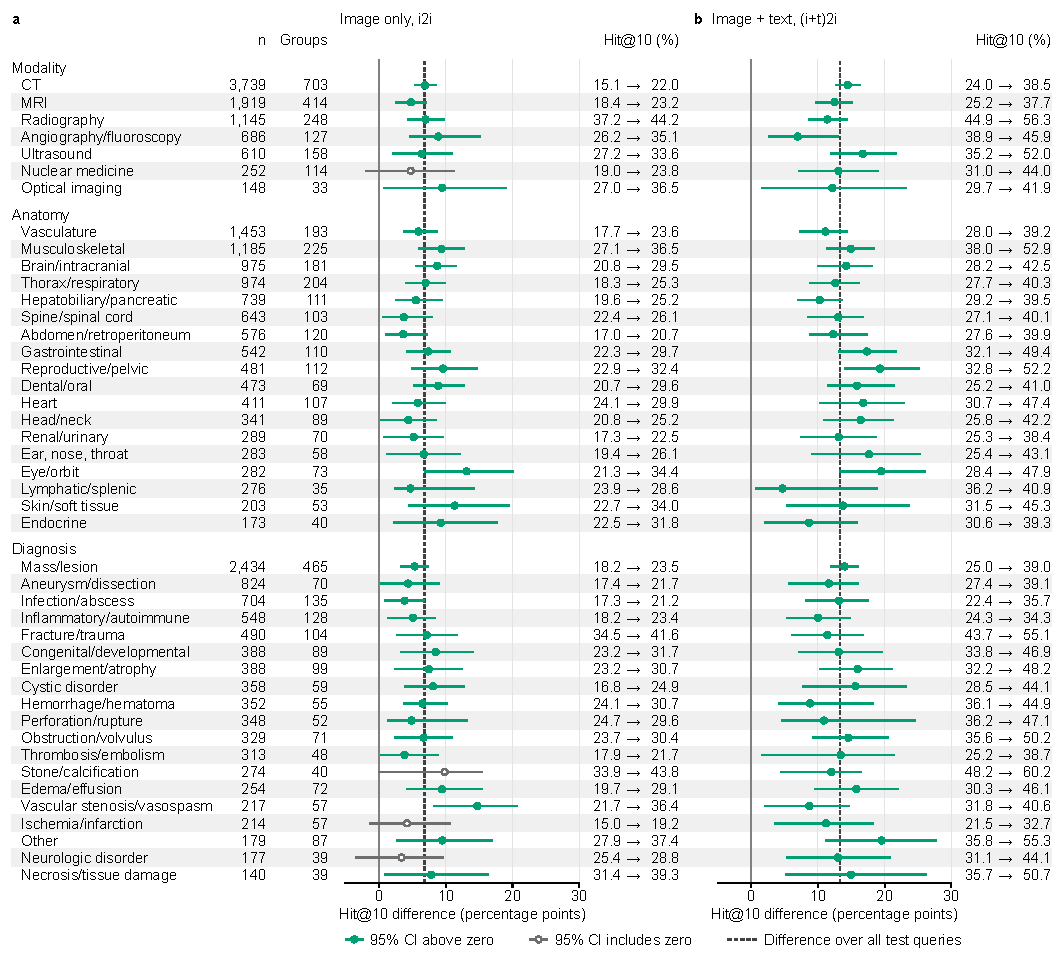
\includegraphics{retrieval_subgroups_hit10.pdf}}
\caption[Change in Hit@10 with fine-tuning across label categories of the 8,096 test queries.]{Change in Hit@10 with fine-tuning across label categories of the 8,096 test queries. Mean Hit@10 is the share of queries with at least one recorded positive partner among their ten highest-ranked images. Each row shows the mean paired difference, fine-tuned minus pretrained, in percentage points. Panel \textbf{a} shows i2i (image-only queries), and panel \textbf{b} shows (i+t)2i (image-plus-text queries). Circles mark mean differences. Lines show 95\% confidence intervals from 5,000 paired bootstrap resamples of article groups, with each query weighted equally. Filled green circles indicate intervals entirely above zero. Open gray circles indicate intervals that include zero. The dashed lines mark the differences over all test queries (+6.84 and +13.30 percentage points, respectively). The columns to the left of panel \textbf{a} give the number of queries ($n$) and article groups represented in each category. These are the groups used to partition the dataset. Numbers to the right of each panel give mean Hit@10 (\%) for the pretrained $\rightarrow$ fine-tuned model. Only categories with at least 140 queries from at least 20 article groups are shown. All categories are listed in \path{results/figures/source_data/subgroups.csv} of the code repository, see Code availability. Categories overlap, and the intervals are not adjusted for multiple comparisons. The results are descriptive. Intervals are approximate when few groups are represented or one group contributes many queries. CI denotes confidence interval, CT denotes computed tomography, and MRI denotes magnetic resonance imaging.}
\label{fig:retrieval-subgroups}
\end{figure}

\begin{figure}[p]
\centering
\makebox[\linewidth][c]{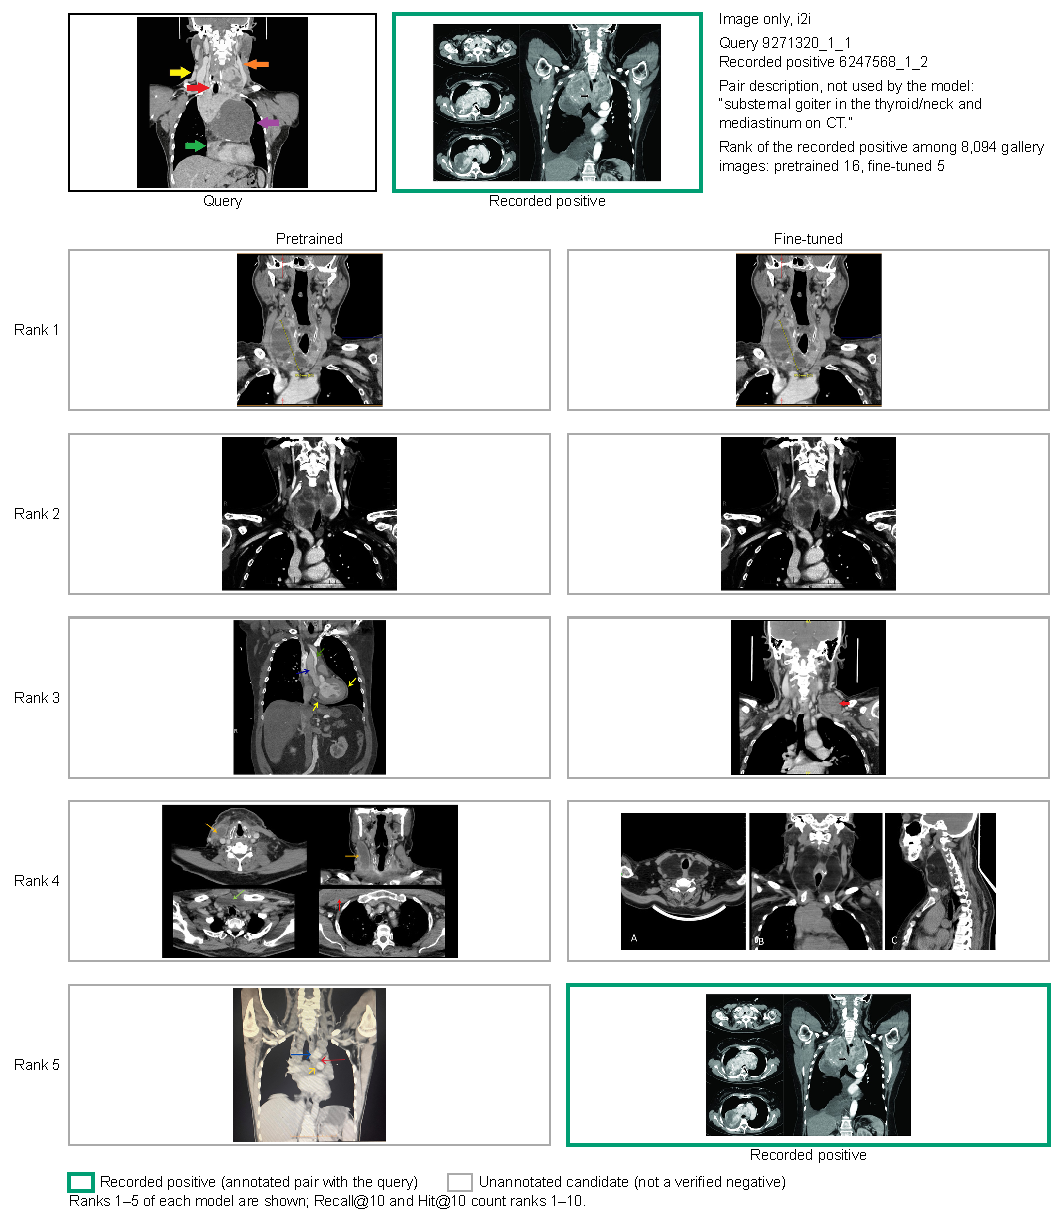
\includegraphics{retrieval_example_improvement_image_to_image.pdf}}
\caption[Retrieval example in which fine-tuning moved the recorded positive into the top five: image-only query, i2i.]{Retrieval example in which fine-tuning moved the recorded positive into the top five: image-only query, i2i. Shown are the test query, its single recorded positive (annotated pair) and the pair description, above the five highest-ranked gallery images of pretrained BiomedCLIP (left) and the fine-tuned model (right; released i2i weights, epoch 11, selected by validation Recall@10); frames and tags as in the key. The recorded positive ranks 16 (pretrained) and 5 (fine-tuned) among the 8,094 ranked gallery images (the other 8,095 test images except 1 linked to the query only through a chain of pairs). Only ranks 1--5 are shown, whereas Recall@10 (share of the query's recorded positives in the top 10) and Hit@10 (any recorded positive in the top 10) count ranks 1--10. The description is composed from the dataset's diagnosis, anatomy and modality fields (\emph{diagnosis} in the \emph{anatomy} on \emph{modality}); CT, computed tomography. Selection: among test queries whose single recorded positive ranks beyond 10 with the pretrained and within the top five with the fine-tuned model and whose displayed images are all openly licensed (Creative Commons Attribution, CC BY, or public domain; commercial reuse, no share-alike), have at least 343 pixels on the longer side and show no burned-in dates, identification numbers, ages or names, the first in ascending order of the SHA-256 hexadecimal digest of \texttt{image\_to\_image/improvement/}\emph{query ID} not selected for an earlier example figure (order: improvement, deterioration, continued miss; image-only first). Images are shown whole, unaltered except for uniform downscaling; letters, arrows and other marks inside them belong to the original figures. Images reproduced from refs.~\cite{PMC9271320,PMC6247568,PMC9019962,PMC8087352,PMC10234142,PMC8544805,PMC12399184,PMC11079707} under CC BY 4.0 (\url{https://creativecommons.org/licenses/by/4.0/}) and ref.~\cite{PMC6857825} under CC BY 3.0 (\url{https://creativecommons.org/licenses/by/3.0/}). The complete selection rule and pool sizes (pmc\_pair\_retrieval/figures.py, results/figures/source\_data/examples.csv) and the images' copyright notices and attributions (results/figures/source\_data/image\_credits.csv) are in the code repository, see Code availability.}
\label{fig:retrieval-example-improvement-image-to-image}
\end{figure}

\begin{figure}[p]
\centering
\makebox[\linewidth][c]{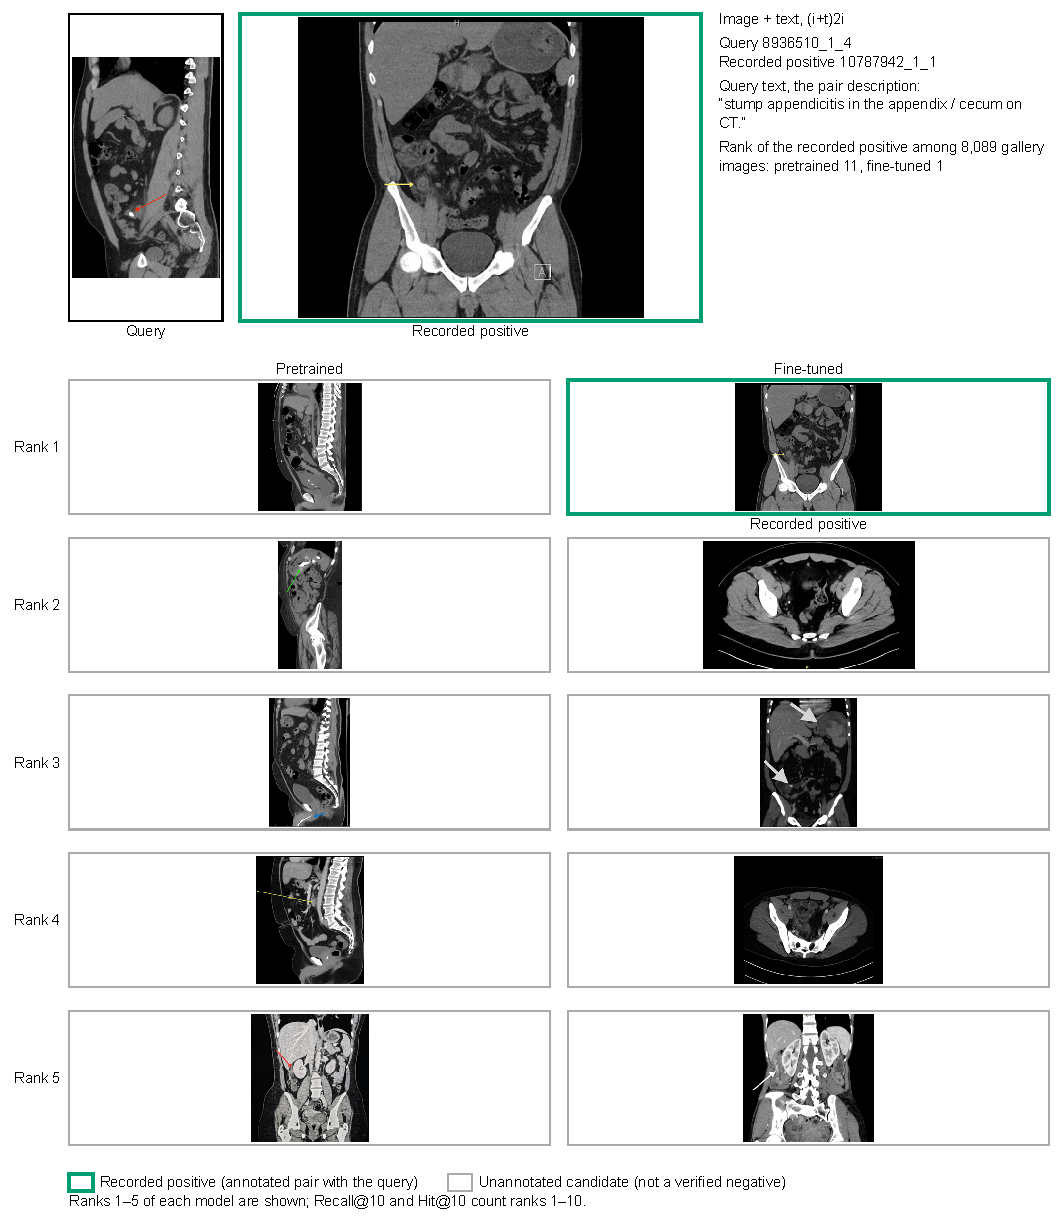
\includegraphics{retrieval_example_improvement_image_text_to_image.pdf}}
\caption[Retrieval example in which fine-tuning moved the recorded positive into the top five: image-plus-text query, (i+t)2i (query image and pair description).]{Retrieval example in which fine-tuning moved the recorded positive into the top five: image-plus-text query, (i+t)2i (query image and pair description). Shown are the test query, its single recorded positive (annotated pair) and the pair description, above the five highest-ranked gallery images of pretrained BiomedCLIP (left) and the fine-tuned model (right; released (i+t)2i weights, epoch 21, selected by validation Recall@10); frames and tags as in the key. The recorded positive ranks 11 (pretrained) and 1 (fine-tuned) among the 8,089 ranked gallery images (the other 8,095 test images except 6 linked to the query only through a chain of pairs). Only ranks 1--5 are shown, whereas Recall@10 (share of the query's recorded positives in the top 10) and Hit@10 (any recorded positive in the top 10) count ranks 1--10. The description is composed from the dataset's diagnosis, anatomy and modality fields (\emph{diagnosis} in the \emph{anatomy} on \emph{modality}); CT, computed tomography. Selection: among test queries whose single recorded positive ranks beyond 10 with the pretrained and within the top five with the fine-tuned model and whose displayed images are all openly licensed (Creative Commons Attribution, CC BY, or public domain; commercial reuse, no share-alike), have at least 343 pixels on the longer side and show no burned-in dates, identification numbers, ages or names, the first in ascending order of the SHA-256 hexadecimal digest of \texttt{image\_text\_to\_image/improvement/}\emph{query ID} not selected for an earlier example figure (order: improvement, deterioration, continued miss; image-only first). Images are shown whole, with their embedded color profiles applied, and otherwise unaltered except for uniform downscaling; letters, arrows and other marks inside them belong to the original figures. Images reproduced from refs.~\cite{PMC8936510,PMC10787942,PMC11138232,PMC8716118,PMC11487295,PMC12712546,PMC12703642,PMC6514724,PMC8612066,PMC8460683,PMC10328655} under CC BY 4.0 (\url{https://creativecommons.org/licenses/by/4.0/}). The complete selection rule and pool sizes (pmc\_pair\_retrieval/figures.py, results/figures/source\_data/examples.csv) and the images' copyright notices and attributions (results/figures/source\_data/image\_credits.csv) are in the code repository, see Code availability.}
\label{fig:retrieval-example-improvement-image-text-to-image}
\end{figure}

\begin{figure}[p]
\centering
\makebox[\linewidth][c]{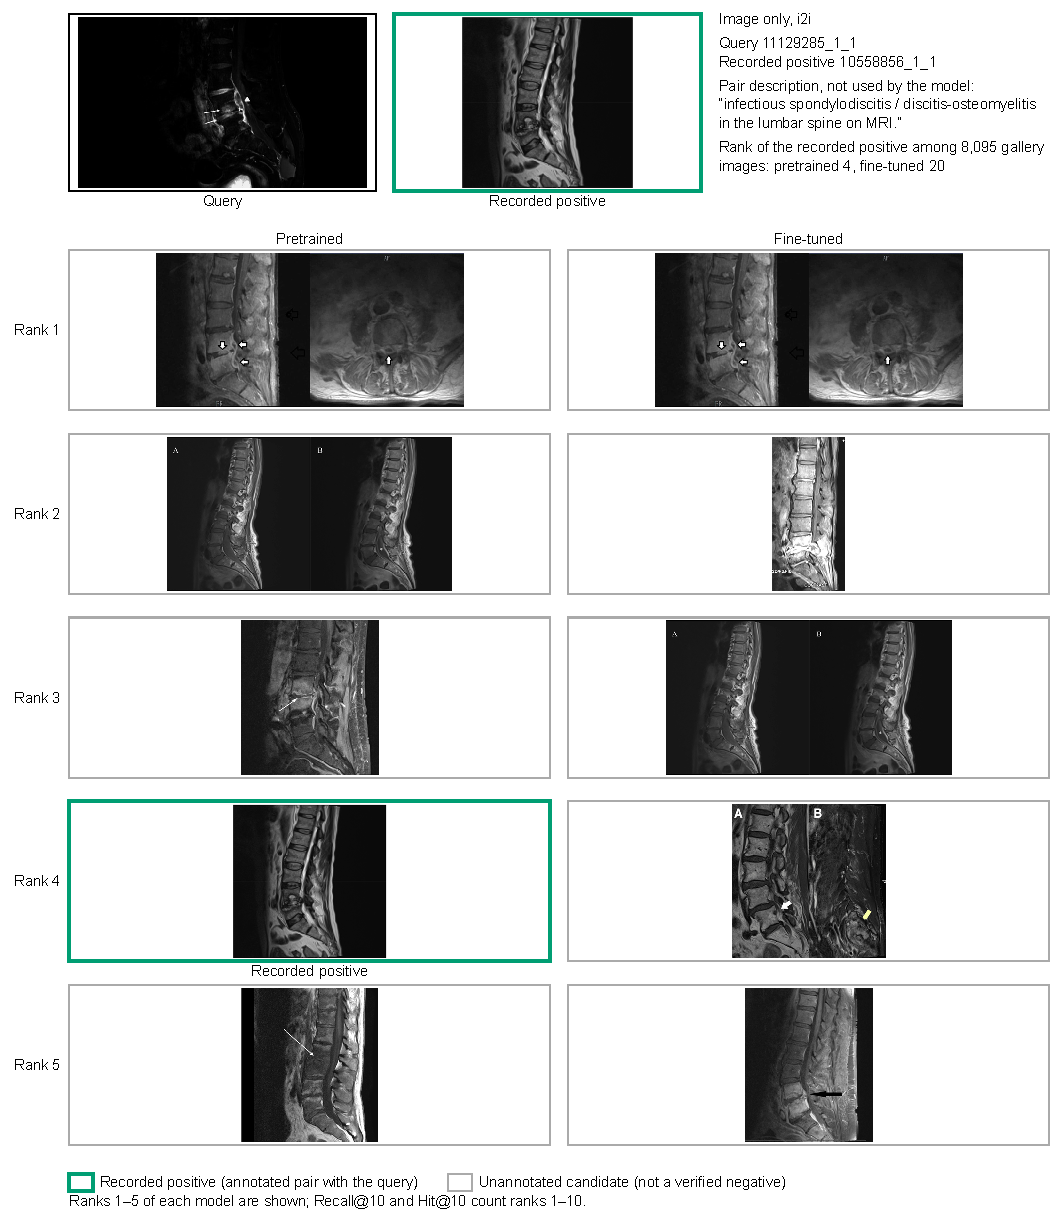
\includegraphics{retrieval_example_deterioration_image_to_image.pdf}}
\caption[Retrieval example in which fine-tuning moved the recorded positive out of the top ten: image-only query, i2i.]{Retrieval example in which fine-tuning moved the recorded positive out of the top ten: image-only query, i2i. Shown are the test query, its single recorded positive (annotated pair) and the pair description, above the five highest-ranked gallery images of pretrained BiomedCLIP (left) and the fine-tuned model (right; released i2i weights, epoch 11, selected by validation Recall@10); frames and tags as in the key. The recorded positive ranks 4 (pretrained) and 20 (fine-tuned) among the 8,095 ranked gallery images (all other test images). Only ranks 1--5 are shown, whereas Recall@10 (share of the query's recorded positives in the top 10) and Hit@10 (any recorded positive in the top 10) count ranks 1--10. The description is composed from the dataset's diagnosis, anatomy and modality fields (\emph{diagnosis} in the \emph{anatomy} on \emph{modality}); MRI, magnetic resonance imaging. Selection: among test queries whose single recorded positive ranks within the top five with the pretrained and beyond 10 with the fine-tuned model and whose displayed images are all openly licensed (Creative Commons Attribution, CC BY, or public domain; commercial reuse, no share-alike), have at least 343 pixels on the longer side and show no burned-in dates, identification numbers, ages or names, the first in ascending order of the SHA-256 hexadecimal digest of \texttt{image\_to\_image/deterioration/}\emph{query ID} not selected for an earlier example figure (order: improvement, deterioration, continued miss; image-only first). Images are shown whole, with their embedded color profiles applied, and otherwise unaltered except for uniform downscaling; letters, arrows and other marks inside them belong to the original figures. Images reproduced from refs.~\cite{PMC11129285,PMC10558856,PMC7402531,PMC10067307,PMC7916262,PMC8793326,PMC10279930,PMC5643001} under CC BY 4.0 (\url{https://creativecommons.org/licenses/by/4.0/}) and ref.~\cite{PMC6314791} under CC BY 3.0 (\url{https://creativecommons.org/licenses/by/3.0/}). The complete selection rule and pool sizes (pmc\_pair\_retrieval/figures.py, results/figures/source\_data/examples.csv) and the images' copyright notices and attributions (results/figures/source\_data/image\_credits.csv) are in the code repository, see Code availability.}
\label{fig:retrieval-example-deterioration-image-to-image}
\end{figure}

\begin{figure}[p]
\centering
\makebox[\linewidth][c]{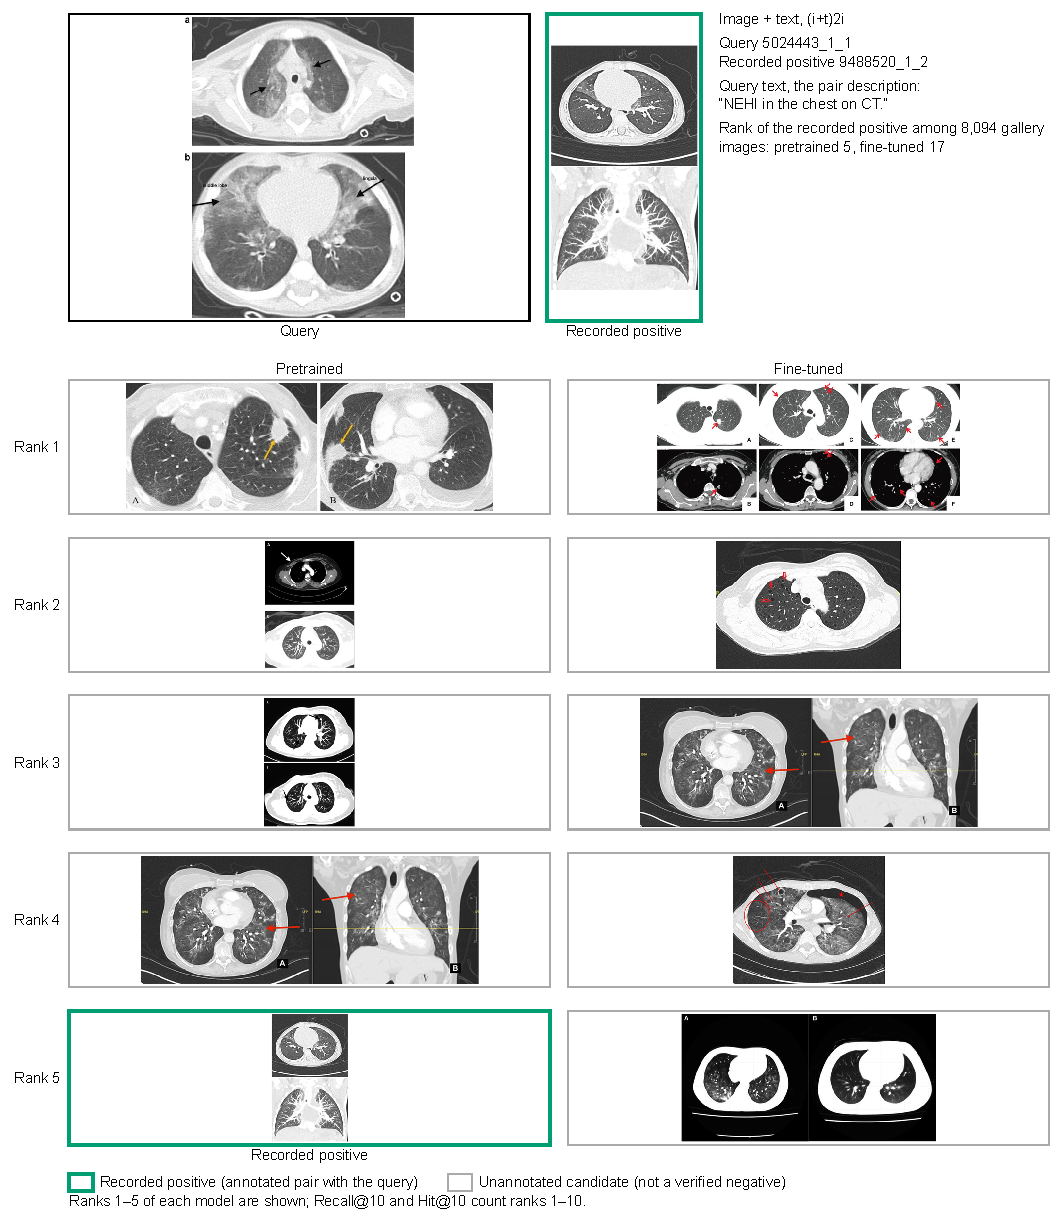
\includegraphics{retrieval_example_deterioration_image_text_to_image.pdf}}
\caption[Retrieval example in which fine-tuning moved the recorded positive out of the top ten: image-plus-text query, (i+t)2i (query image and pair description).]{Retrieval example in which fine-tuning moved the recorded positive out of the top ten: image-plus-text query, (i+t)2i (query image and pair description). Shown are the test query, its single recorded positive (annotated pair) and the pair description, above the five highest-ranked gallery images of pretrained BiomedCLIP (left) and the fine-tuned model (right; released (i+t)2i weights, epoch 21, selected by validation Recall@10); frames and tags as in the key. The recorded positive ranks 5 (pretrained) and 17 (fine-tuned) among the 8,094 ranked gallery images (the other 8,095 test images except 1 linked to the query only through a chain of pairs). Only ranks 1--5 are shown, whereas Recall@10 (share of the query's recorded positives in the top 10) and Hit@10 (any recorded positive in the top 10) count ranks 1--10. The description is composed from the dataset's diagnosis, anatomy and modality fields (\emph{diagnosis} in the \emph{anatomy} on \emph{modality}); NEHI, neuroendocrine cell hyperplasia of infancy; CT, computed tomography. Selection: among test queries whose single recorded positive ranks within the top five with the pretrained and beyond 10 with the fine-tuned model and whose displayed images are all openly licensed (Creative Commons Attribution, CC BY, or public domain; commercial reuse, no share-alike), have at least 343 pixels on the longer side and show no burned-in dates, identification numbers, ages or names, the first in ascending order of the SHA-256 hexadecimal digest of \texttt{image\_text\_to\_image/deterioration/}\emph{query ID} not selected for an earlier example figure (order: improvement, deterioration, continued miss; image-only first). Images are shown whole, unaltered except for uniform downscaling; letters, arrows and other marks inside them belong to the original figures. Images reproduced from refs.~\cite{PMC5024443,PMC9488520,PMC10834218,PMC11228424,PMC10859509,PMC11186622,PMC11266077} under CC BY 4.0 (\url{https://creativecommons.org/licenses/by/4.0/}) and refs.~\cite{PMC6663116,PMC6433088} under CC BY 3.0 (\url{https://creativecommons.org/licenses/by/3.0/}). The complete selection rule and pool sizes (pmc\_pair\_retrieval/figures.py, results/figures/source\_data/examples.csv) and the images' copyright notices and attributions (results/figures/source\_data/image\_credits.csv) are in the code repository, see Code availability.}
\label{fig:retrieval-example-deterioration-image-text-to-image}
\end{figure}

\begin{figure}[p]
\centering
\makebox[\linewidth][c]{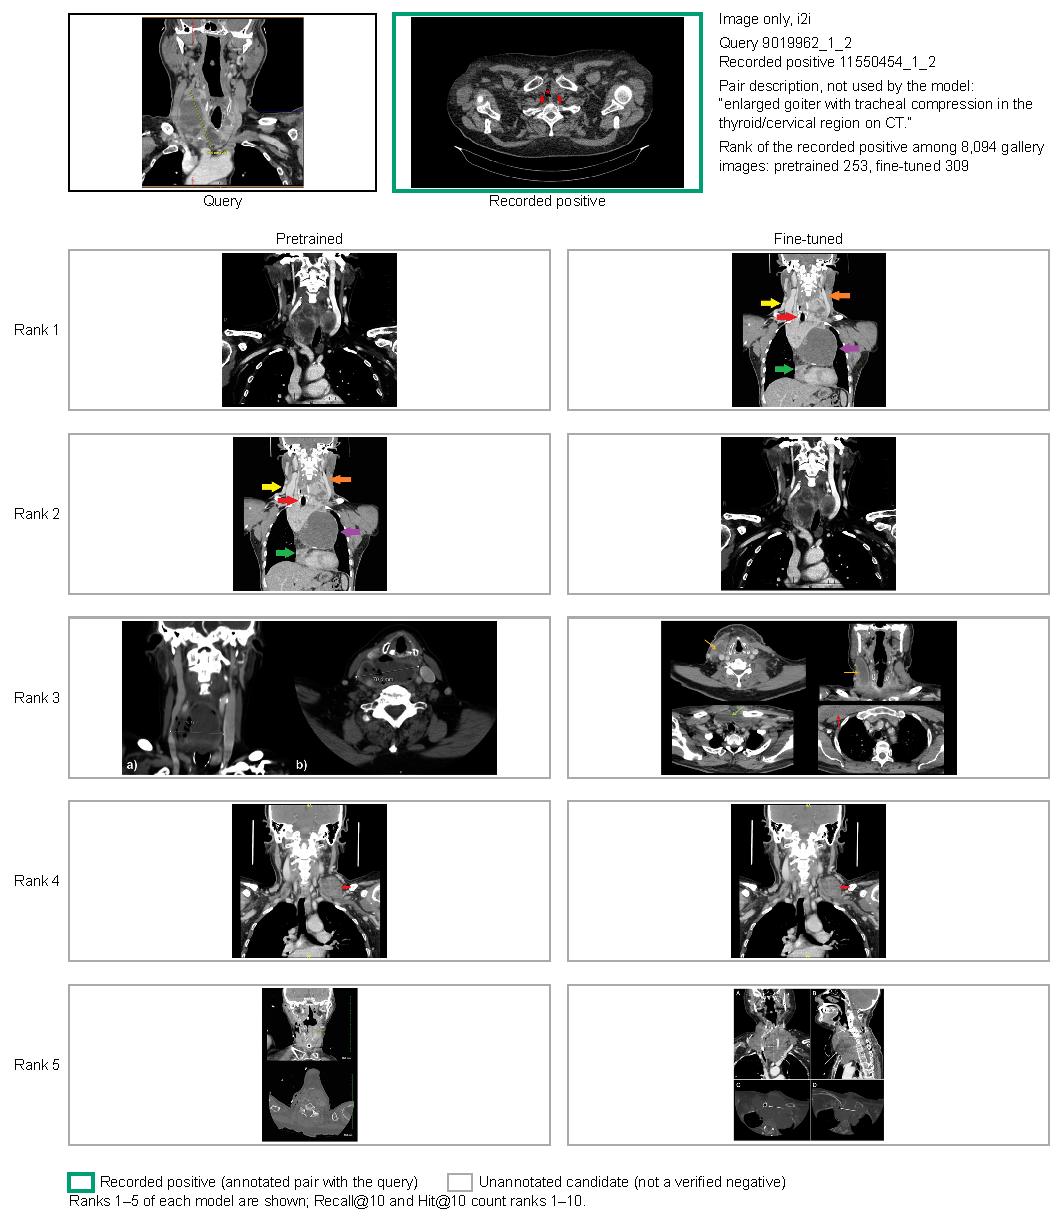
\includegraphics{retrieval_example_continued_miss_image_to_image.pdf}}
\caption[Retrieval example in which neither model ranks the recorded positive in the top ten: image-only query, i2i.]{Retrieval example in which neither model ranks the recorded positive in the top ten: image-only query, i2i. Shown are the test query, its single recorded positive (annotated pair) and the pair description, above the five highest-ranked gallery images of pretrained BiomedCLIP (left) and the fine-tuned model (right; released i2i weights, epoch 11, selected by validation Recall@10); frames and tags as in the key. The recorded positive ranks 253 (pretrained) and 309 (fine-tuned) among the 8,094 ranked gallery images (the other 8,095 test images except 1 linked to the query only through a chain of pairs). Only ranks 1--5 are shown, whereas Recall@10 (share of the query's recorded positives in the top 10) and Hit@10 (any recorded positive in the top 10) count ranks 1--10. The description is composed from the dataset's diagnosis, anatomy and modality fields (\emph{diagnosis} in the \emph{anatomy} on \emph{modality}); CT, computed tomography. Selection: among test queries whose single recorded positive ranks beyond 10 with both models and whose displayed images are all openly licensed (Creative Commons Attribution, CC BY, or public domain; commercial reuse, no share-alike), have at least 343 pixels on the longer side and show no burned-in dates, identification numbers, ages or names, the first in ascending order of the SHA-256 hexadecimal digest of \texttt{image\_to\_image/continued\_miss/}\emph{query ID} not selected for an earlier example figure (order: improvement, deterioration, continued miss; image-only first). Images are shown whole, unaltered except for uniform downscaling; letters, arrows and other marks inside them belong to the original figures. Images reproduced from refs.~\cite{PMC9019962,PMC11550454,PMC8087352,PMC9271320,PMC10696619,PMC5345263,PMC8544805,PMC12352973} under CC BY 4.0 (\url{https://creativecommons.org/licenses/by/4.0/}) and ref.~\cite{PMC6857825} under CC BY 3.0 (\url{https://creativecommons.org/licenses/by/3.0/}). The complete selection rule and pool sizes (pmc\_pair\_retrieval/figures.py, results/figures/source\_data/examples.csv) and the images' copyright notices and attributions (results/figures/source\_data/image\_credits.csv) are in the code repository, see Code availability.}
\label{fig:retrieval-example-continued-miss-image-to-image}
\end{figure}

\begin{figure}[p]
\centering
\makebox[\linewidth][c]{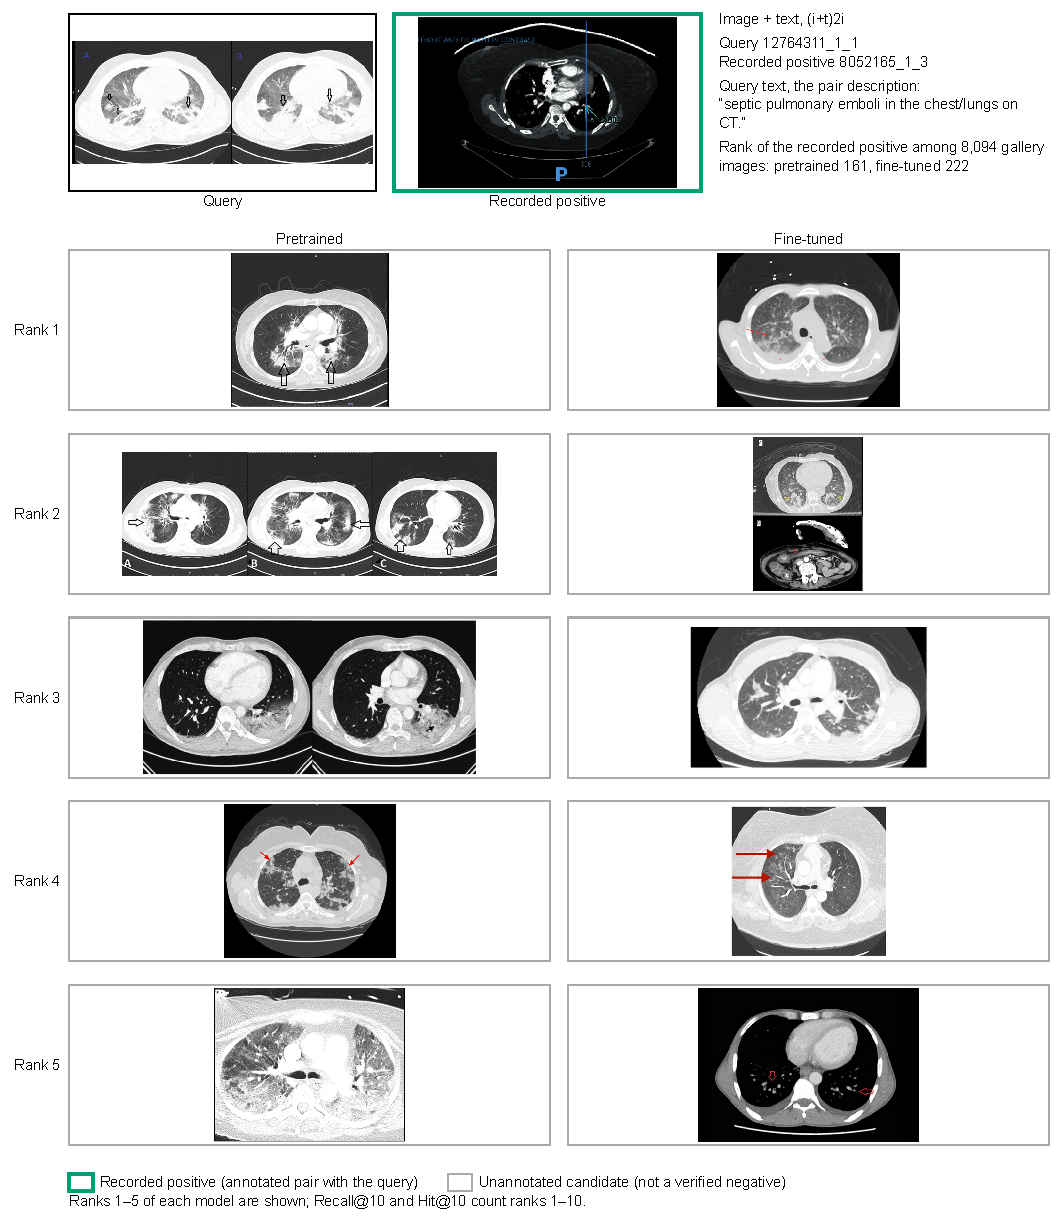
\includegraphics{retrieval_example_continued_miss_image_text_to_image.pdf}}
\caption[Retrieval example in which neither model ranks the recorded positive in the top ten: image-plus-text query, (i+t)2i (query image and pair description).]{Retrieval example in which neither model ranks the recorded positive in the top ten: image-plus-text query, (i+t)2i (query image and pair description). Shown are the test query, its single recorded positive (annotated pair) and the pair description, above the five highest-ranked gallery images of pretrained BiomedCLIP (left) and the fine-tuned model (right; released (i+t)2i weights, epoch 21, selected by validation Recall@10); frames and tags as in the key. The recorded positive ranks 161 (pretrained) and 222 (fine-tuned) among the 8,094 ranked gallery images (the other 8,095 test images except 1 linked to the query only through a chain of pairs). Only ranks 1--5 are shown, whereas Recall@10 (share of the query's recorded positives in the top 10) and Hit@10 (any recorded positive in the top 10) count ranks 1--10. The description is composed from the dataset's diagnosis, anatomy and modality fields (\emph{diagnosis} in the \emph{anatomy} on \emph{modality}); CT, computed tomography. Selection: among test queries whose single recorded positive ranks beyond 10 with both models and whose displayed images are all openly licensed (Creative Commons Attribution, CC BY, or public domain; commercial reuse, no share-alike), have at least 343 pixels on the longer side and show no burned-in dates, identification numbers, ages or names, the first in ascending order of the SHA-256 hexadecimal digest of \texttt{image\_text\_to\_image/continued\_miss/}\emph{query ID} not selected for an earlier example figure (order: improvement, deterioration, continued miss; image-only first). Images are shown whole, unaltered except for uniform downscaling; letters, arrows and other marks inside them belong to the original figures. Images reproduced from refs.~\cite{PMC12764311,PMC8052165,PMC10276897,PMC11099301,PMC10234608,PMC6186889,PMC8752349,PMC7440261,PMC4835622,PMC9937636} under CC BY 4.0 (\url{https://creativecommons.org/licenses/by/4.0/}) and ref.~\cite{PMC7034735} under CC BY 3.0 (\url{https://creativecommons.org/licenses/by/3.0/}). The complete selection rule and pool sizes (pmc\_pair\_retrieval/figures.py, results/figures/source\_data/examples.csv) and the images' copyright notices and attributions (results/figures/source\_data/image\_credits.csv) are in the code repository, see Code availability.}
\label{fig:retrieval-example-continued-miss-image-text-to-image}
\end{figure}
